%%% figure_main.tex

\documentclass[border=3mm]{standalone}

\usepackage{tikz}
\usetikzlibrary{shapes.arrows,decorations.pathreplacing,arrows.meta}

\tikzset{
    double -latex/.style args={#1 colored by #2 and #3}{    
        -{Triangle[length=0.5cm,width=0.92cm]},line width=#1,#2,
        postaction={draw,-{Triangle[length=0.46cm,width=0.84cm]},#3,line width=(#1)-2*0.2mm,
            shorten <=0.2mm, shorten >=0.22mm)},
    },
}

\usepackage{graphicx}

\definecolor{myBlue}{RGB}{15,158,213}
\definecolor{myPurple}{RGB}{160,43,147}
\definecolor{myOrange}{RGB}{233,113,50}

\begin{document}
	\begin{tikzpicture}
		\node[label={above,align=center:Prediction models},draw,rectangle,rounded corners=5pt] (A) at (-6,0) {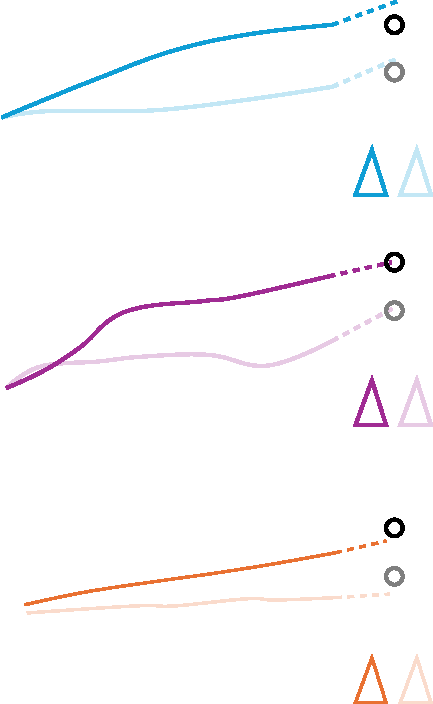
\includegraphics[scale=0.5]{images/part-1.pdf}};
		\node[single arrow,draw,minimum height=10mm] at (-2.75,0){};
		\node[label={above,align=center:Parameter\\quasi-posterior}] (B) at (0,0) {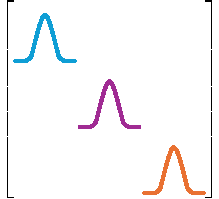
\includegraphics{images/part-2.pdf}};
		\node[single arrow,draw,minimum height=10mm] at (2.75,0){};
		\node[label={above:Parameter draws}] (C) at (6,0) {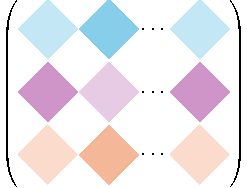
\includegraphics{images/part-3.pdf}};
		\node[single arrow,draw,minimum height=10mm,rotate=-90] at (6,-2.5){};
		\node[scale=1.6,draw,rectangle,rounded corners=5pt,label={right,align=center:Min-max differential prediction\\errors (in validation periods)}] (D) at (2,-6.5) {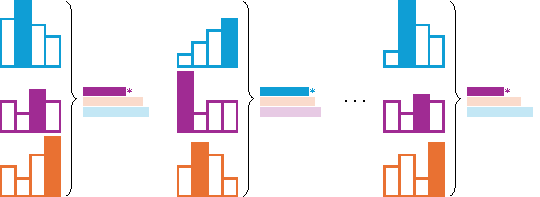
\includegraphics{images/part-4.pdf}};
		\draw[decorate,decoration={brace,amplitude=5pt,mirror}] ([yshift=-1pt]D.south west) -- ([yshift=-1pt]D.south east) node[midway,below,label={left,align=center:Quasi-posterior\\model probabilities}](E){
\includegraphics{images/part-5.pdf}};
		\node[scale=0.75,label={below,align=center:Bayesian model-averaged estimate\\(in post-treatment period)}](F) at (8.5,-13) {
\includegraphics{images/part-6.pdf}};
		\draw[double -latex=3mm colored by black and white] (E.south) |- (F.west);
	\end{tikzpicture}
\end{document}